% Options for packages loaded elsewhere
% Options for packages loaded elsewhere
\PassOptionsToPackage{unicode}{hyperref}
\PassOptionsToPackage{hyphens}{url}
\PassOptionsToPackage{dvipsnames,svgnames,x11names}{xcolor}
%
\documentclass[
  japanese,
  11pt,
  letterpaper,
  DIV=11,
  numbers=noendperiod]{scrartcl}
\usepackage{xcolor}
\usepackage[margin=25mm,top=25mm,bottom=25mm,left=20mm,right=20mm]{geometry}
\usepackage{amsmath,amssymb}
\setcounter{secnumdepth}{-\maxdimen} % remove section numbering
\usepackage{iftex}
\ifPDFTeX
  \usepackage[T1]{fontenc}
  \usepackage[utf8]{inputenc}
  \usepackage{textcomp} % provide euro and other symbols
\else % if luatex or xetex
  \usepackage{unicode-math} % this also loads fontspec
  \defaultfontfeatures{Scale=MatchLowercase}
  \defaultfontfeatures[\rmfamily]{Ligatures=TeX,Scale=1}
\fi
\usepackage{lmodern}
\ifPDFTeX\else
  % xetex/luatex font selection
\fi
% Use upquote if available, for straight quotes in verbatim environments
\IfFileExists{upquote.sty}{\usepackage{upquote}}{}
\IfFileExists{microtype.sty}{% use microtype if available
  \usepackage[]{microtype}
  \UseMicrotypeSet[protrusion]{basicmath} % disable protrusion for tt fonts
}{}
\usepackage{setspace}
\makeatletter
\@ifundefined{KOMAClassName}{% if non-KOMA class
  \IfFileExists{parskip.sty}{%
    \usepackage{parskip}
  }{% else
    \setlength{\parindent}{0pt}
    \setlength{\parskip}{6pt plus 2pt minus 1pt}}
}{% if KOMA class
  \KOMAoptions{parskip=half}}
\makeatother
% Make \paragraph and \subparagraph free-standing
\makeatletter
\ifx\paragraph\undefined\else
  \let\oldparagraph\paragraph
  \renewcommand{\paragraph}{
    \@ifstar
      \xxxParagraphStar
      \xxxParagraphNoStar
  }
  \newcommand{\xxxParagraphStar}[1]{\oldparagraph*{#1}\mbox{}}
  \newcommand{\xxxParagraphNoStar}[1]{\oldparagraph{#1}\mbox{}}
\fi
\ifx\subparagraph\undefined\else
  \let\oldsubparagraph\subparagraph
  \renewcommand{\subparagraph}{
    \@ifstar
      \xxxSubParagraphStar
      \xxxSubParagraphNoStar
  }
  \newcommand{\xxxSubParagraphStar}[1]{\oldsubparagraph*{#1}\mbox{}}
  \newcommand{\xxxSubParagraphNoStar}[1]{\oldsubparagraph{#1}\mbox{}}
\fi
\makeatother


\usepackage{longtable,booktabs,array}
\usepackage{calc} % for calculating minipage widths
% Correct order of tables after \paragraph or \subparagraph
\usepackage{etoolbox}
\makeatletter
\patchcmd\longtable{\par}{\if@noskipsec\mbox{}\fi\par}{}{}
\makeatother
% Allow footnotes in longtable head/foot
\IfFileExists{footnotehyper.sty}{\usepackage{footnotehyper}}{\usepackage{footnote}}
\makesavenoteenv{longtable}
\usepackage{graphicx}
\makeatletter
\newsavebox\pandoc@box
\newcommand*\pandocbounded[1]{% scales image to fit in text height/width
  \sbox\pandoc@box{#1}%
  \Gscale@div\@tempa{\textheight}{\dimexpr\ht\pandoc@box+\dp\pandoc@box\relax}%
  \Gscale@div\@tempb{\linewidth}{\wd\pandoc@box}%
  \ifdim\@tempb\p@<\@tempa\p@\let\@tempa\@tempb\fi% select the smaller of both
  \ifdim\@tempa\p@<\p@\scalebox{\@tempa}{\usebox\pandoc@box}%
  \else\usebox{\pandoc@box}%
  \fi%
}
% Set default figure placement to htbp
\def\fps@figure{htbp}
\makeatother



\ifLuaTeX
\usepackage[bidi=basic,provide=*]{babel}
\else
\usepackage[bidi=default,provide=*]{babel}
\fi
% get rid of language-specific shorthands (see #6817):
\let\LanguageShortHands\languageshorthands
\def\languageshorthands#1{}


\setlength{\emergencystretch}{3em} % prevent overfull lines

\providecommand{\tightlist}{%
  \setlength{\itemsep}{0pt}\setlength{\parskip}{0pt}}



 


\usepackage{booktabs}
\usepackage{caption}
\usepackage{longtable}
\usepackage{colortbl}
\usepackage{array}
\usepackage{anyfontsize}
\usepackage{multirow}
\usepackage{luatexja}
\usepackage[haranoaji]{luatexja-preset}
\usepackage{fontspec}\setmainfont{TeX Gyre Termes}
\usepackage{caption}\captionsetup[table]{skip=6pt}
\usepackage{booktabs,longtable,array,xcolor,colortbl,multirow}
\usepackage{pdflscape}
\newcommand{\blandscape}{\begin{landscape}}
\newcommand{\elandscape}{\end{landscape}}
\KOMAoption{captions}{tableheading}
\usepackage{titlesec}
\usepackage{xcolor}
\usepackage{caption}
\captionsetup[table]{name=Table,labelsep=period}
\captionsetup[figure]{name=Fig,labelsep=period}
% 見出し後の共通余白を定義
\newlength{\headingafter}
\setlength{\headingafter}{0ex}
%{0ex plus 0.4ex minus 0.2ex}

% ----- section -----
\titleformat{\section}
  {\normalfont\large\bfseries\centering\color{black}}
  {\thesection}{1em}{}
\titlespacing*{\section}
  {0pt}          % 左インデント
  {2.5ex plus 1ex} % 見出しの「前（上）」の余白（レベルごとに変えてOK）
  {\headingafter}  % 見出しの「後（下）」＝本文との行間（共通）

% ----- subsection -----
\titleformat{\subsection}
  {\normalfont\large\bfseries\color{black}}
  {\thesubsection}{0.7em}{}
\titlespacing*{\subsection}
  {0pt}          % 左インデント
  {2.5ex plus 1ex} % 見出しの「前（上）」の余白（レベルごとに変えてOK）
  {\headingafter}  % 見出しの「後（下）」＝本文との行間（共通）

% ----- subsubsection -----
\titleformat{\subsubsection}
  {\normalfont\normalsize\bfseries\color{black}}
  {\thesubsubsection}{0.5em}{}
\titlespacing*{\subsubsection}
  {0pt}          % 左インデント
  {2.5ex plus 1ex} % 見出しの「前（上）」の余白（レベルごとに変えてOK）
  {\headingafter}  % 見出しの「後（下）」＝本文との行間（共通）
\makeatletter
\@ifpackageloaded{caption}{}{\usepackage{caption}}
\AtBeginDocument{%
\ifdefined\contentsname
  \renewcommand*\contentsname{目次}
\else
  \newcommand\contentsname{目次}
\fi
\ifdefined\listfigurename
  \renewcommand*\listfigurename{図一覧}
\else
  \newcommand\listfigurename{図一覧}
\fi
\ifdefined\listtablename
  \renewcommand*\listtablename{表一覧}
\else
  \newcommand\listtablename{表一覧}
\fi
\ifdefined\figurename
  \renewcommand*\figurename{図}
\else
  \newcommand\figurename{図}
\fi
\ifdefined\tablename
  \renewcommand*\tablename{表}
\else
  \newcommand\tablename{表}
\fi
}
\@ifpackageloaded{float}{}{\usepackage{float}}
\floatstyle{ruled}
\@ifundefined{c@chapter}{\newfloat{codelisting}{h}{lop}}{\newfloat{codelisting}{h}{lop}[chapter]}
\floatname{codelisting}{コード}
\newcommand*\listoflistings{\listof{codelisting}{コード一覧}}
\makeatother
\makeatletter
\makeatother
\makeatletter
\@ifpackageloaded{caption}{}{\usepackage{caption}}
\@ifpackageloaded{subcaption}{}{\usepackage{subcaption}}
\makeatother
\usepackage{bookmark}
\IfFileExists{xurl.sty}{\usepackage{xurl}}{} % add URL line breaks if available
\urlstyle{same}
\hypersetup{
  pdftitle={アサノ大成基礎エンジニアリング報告書},
  pdfauthor={名前 大学},
  pdflang={ja},
  colorlinks=true,
  linkcolor={blue},
  filecolor={Maroon},
  citecolor={Blue},
  urlcolor={Blue},
  pdfcreator={LaTeX via pandoc}}


\title{アサノ大成基礎エンジニアリング報告書}
\author{名前 大学}
\date{}
\begin{document}
\maketitle


\setstretch{1.5}
\newpage

\section{目的}\label{ux76eeux7684}

　CO\textsubscript{2}排出量の削減は世界規模の課題であり，我が国においても2050年までのカーボンニュートラルの達成が目標となっている。施設園芸では一般的に冬季には化石燃料由来のエネルギーによって，温室を暖房することが一般的に行われており，施設園芸における園芸作物生産はCO\textsubscript{2}の大幅な排出が伴うことから，この排出量の削減が大きな課題となっている。したがって，再生可能エネルギーおよび低利用エネルギーの積極的な利用を見据えた省エネルギー・低CO\textsubscript{2}排出栽培技術の開発が必要である。そこで，本研究ではアサノ大成基礎エンジニアリング株式会社が得意とする地中熱利用と日本大学が開発中の蓄熱型N.RECS（N.RECS-hs）を組み合わせて，省エネルギー・脱炭素型植物栽培システムを構築するとともに，従来方法と比較して本システムの性能を評価することを目的とする。

\section{材料および方法}\label{ux6750ux6599ux304aux3088ux3073ux65b9ux6cd5}

\subsection{温室内における装置の配置と運用}\label{ux6e29ux5ba4ux5185ux306bux304aux3051ux308bux88c5ux7f6eux306eux914dux7f6eux3068ux904bux7528}

　日本大学生物資源科学部のフェンロー型プラスチック温室を東西に二分割し，東側を対照温室，西側を処理温室とした。
に処理温室内におけるに熱源と各種N.RECS栽培装置の設置状況およびセンサーの設置位置を示した（
Fig~\ref{fig-greenhouse} ）。同温室内には幅1.3 m，長さ9
mの栽培ベンチが南北に3台ずつ，合計６台設置されている。北側と南側のベンチには，それぞれ標準型N.RECS（N.RECS-st），蓄熱型N.RECS-hs（N.RECS-hs），U字溝型N.RECS(N.RECS-ug）を導入した。
　N.RECS-stとN.RECS-hsの栽培槽の内寸は幅0.9 m，長さ6
mであるがPEX管のリターン部分を調整するためアルミ製熱交換パネルは5mの長さとしたため，実効栽培面積は4.5
m\textsuperscript{2}であった。N.RECS-stにおける根域温度の制御はスマートガーデナー（オネスト）により行った。N.RECS-hsはN.RECS-stの栽培槽の下にN.RECS-stの実効栽培面積と同一の蓄熱槽を設置した。この蓄熱部分は外寸10
× 10 × 100 cmのアルミ製カートリッジ45本からなり，各カートリッジには8
Lの水を充填した。このカートリッジの上下をアルミ製熱交換パネルで挟みPEX管に冷温水を送液した。熱源から蓄熱槽および蓄熱槽から栽培槽への送液制御は，オネスト社製の制御装置により行った。N.RECS-ugは内寸0.2
m，長さ8
mのものを一つのベンチに2本設置した。根域温度の制御はN.RECS-stと同様にスマートガーデナーで行った。N.RECS用熱源は北側3ベンチを地下水熱式ヒートポンプ，南側3ベンチを空気熱源式ヒートポンプとした。熱源とN.RECSへの接続は並列とし，熱源からN.RECSまでの配管距離はほぼ同一であった。

\begin{figure}[H]

\centering{

\pandocbounded{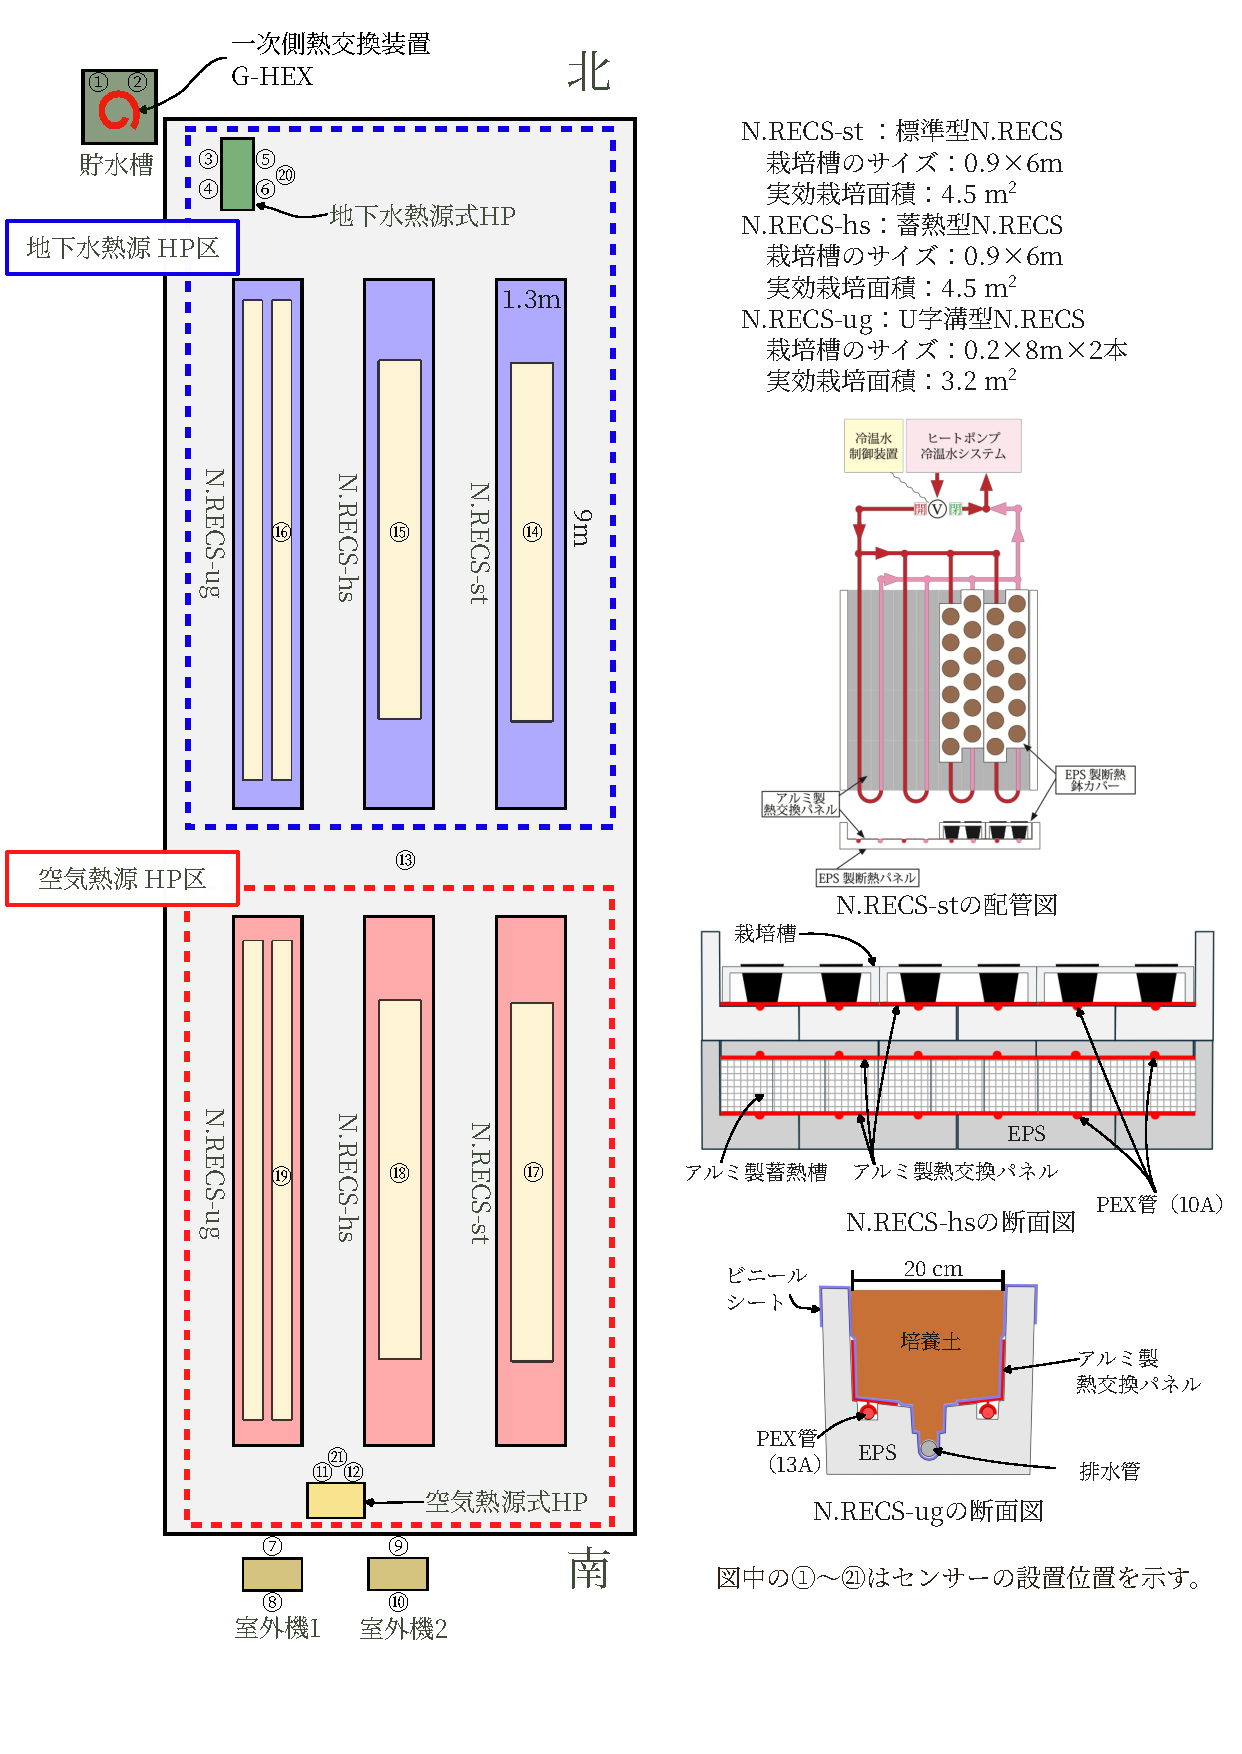
\includegraphics[keepaspectratio]{../figs/greenhouse20251117.pdf}}

}

\caption{\label{fig-greenhouse}処理区における温室内の実験区の配置}

\end{figure}%

\subsection{供試したヒートポンプの種類と性能}\label{ux4f9bux8a66ux3057ux305fux30d2ux30fcux30c8ux30ddux30f3ux30d7ux306eux7a2eux985eux3068ux6027ux80fd}

　ヒートポンプ（HP）の種類と設定 空気熱源式HP（Air
HP）にはエコヌクールレオ（三菱電機（株），VEH-712HCC-k），地下水熱源式HP（Water
HP）には（（株）長府製作所，GSHP-0624X）を用いた。Air
HPの一次側熱交換器（室外機）は温室南側の外に設置し，Water
HPの一次側熱交換は温室北西に設置した貯水槽内に設置した未利用熱回収用熱交換ユニット（ジオシステム（株），G-HEX）に接続して行った。貯水槽には日本大学生物資源科学部の井戸水を供給し，供給のタイミングはスマートガーデナーで制御した。
Table~\ref{tbl-spec} に両熱源の主要諸元を示した。Air HPの冷却能力は7.2
kW，定格消費電力は2.57 kW，Water HPの冷却能力は6.0
kW，定格消費電力は1.33
kWであり，両熱源の計算上のCOPはそれぞれ2.80と4.51であった。

\begin{table}[H]

\caption{\label{tbl-spec}熱源の諸元}

\centering{

\fontsize{12.0pt}{14.0pt}\selectfont
\begin{tabular*}{\linewidth}{@{\extracolsep{\fill}}llcccc}
\toprule
 &  & \multicolumn{2}{c}{冷却（kW）} & \multicolumn{2}{c}{加熱（kW）} \\ 
\cmidrule(lr){3-4} \cmidrule(lr){5-6}
{熱源} & {型式} & 能力 & 定格消費電力 & 能力 & 定格消費電力 \\ 
\midrule\addlinespace[2.5pt]
空気熱源 & VEH-712HCC-k & 7.2 & 2.57 & 11.8 & 2.95 \\ 
地下水熱源 & GSHP-0624X & 6.0 & 1.33 & 6.0 & 1.14 \\ 
\bottomrule
\end{tabular*}

}

\end{table}%

\subsection{各部位の温度と流速測定に用いたセンサーと消費電力量の計測}\label{ux5404ux90e8ux4f4dux306eux6e29ux5ea6ux3068ux6d41ux901fux6e2cux5b9aux306bux7528ux3044ux305fux30bbux30f3ux30b5ux30fcux3068ux6d88ux8cbbux96fbux529bux91cfux306eux8a08ux6e2c}

　温度等のセンサーの設置位置はに示し，それらのセンサーの測定対象と種類等については
Table~\ref{tbl-sensorID1} と Table~\ref{tbl-sensorID2}
に示した。各種温度についてはサーミスタまたはPt100，両熱源の二次側流速は小型電磁流量センサー（愛知時計電機（株），VN10R）で計測した。全ての計測データは1分間隔でデータロガーに記録した。両熱源の消費電力量は小型電力モニタ（オムロン（株），KM-N1-FLK）で計測し，そのパルス出力をデータロガー（ティアンドデイ（株），RTR505B）で1分間ごとに記録した。
記録したデータはRで作成したスクリプトにより適宜成形した後mysqlサーバーにアップロードし，異なるセンサーのデータを連結して適宜図を作成した。なお，Pt100の測定データの一部にノイズが見られたので，Rで作成したHampel関数によりノイズを除去した。

\clearpage
\blandscape

\begin{table}[H]

\caption{\label{tbl-sensorID1}センサーの設置場所，測定対象とセンサーの種類-1}

\centering{

\fontsize{12.0pt}{14.0pt}\selectfont
\begin{tabular*}{\linewidth}{@{\extracolsep{\fill}}clllll}
\toprule
センサー番号 & 設置場所 & 測定対象 & センサーの種類 & メーカー & 測定開始日 \\ 
\midrule\addlinespace[2.5pt]
① & 貯水槽 & 貯水槽水温 & サーミスタ & （株）オネスト & 2025年8月日 \\ 
② & 貯水槽 & 井戸水供給水温 & サーミスタ & （株）オネスト & 2025年8月日 \\ 
③ & 地下水熱源式HP & 一次側行き水温 & Pt100 & ATE様提供品 & 2025年8月日 \\ 
④ & 地下水熱源式HP & 一次側戻り水温 & Pt100 & ATE様提供品 & 2025年8月日 \\ 
⑤ & 地下水熱源式HP & 二次側行き水温 & サーミスタ & （株）ティアンドデイ & 2025年8月日 \\ 
⑥ & 地下水熱源式HP & 二次側戻り水温 & サーミスタ & （株）ティアンドデイ & 2025年8月日 \\ 
\shortstack[l]{⑦ \\　} & \shortstack[l]{空気熱源式HP \\　} & \shortstack[l]{室外機1 \\吸気側気温} & \shortstack[l]{サーミスタ \\　} & \shortstack[l]{（株）ティアンドデイ \\　} & \shortstack[l]{2025年8月日 \\　} \\ 
\shortstack[l]{⑧ \\　} & \shortstack[l]{空気熱源式HP \\　} & \shortstack[l]{室外機1 \\排気側気温} & \shortstack[l]{サーミスタ \\　} & \shortstack[l]{（株）ティアンドデイ \\　} & \shortstack[l]{2025年8月日 \\　} \\ 
\shortstack[l]{⑨ \\　} & \shortstack[l]{空気熱源式HP \\　} & \shortstack[l]{室外機2 \\吸気側気温} & \shortstack[l]{サーミスタ \\　} & \shortstack[l]{（株）ティアンドデイ \\　} & \shortstack[l]{2025年8月日 \\　} \\ 
\shortstack[l]{⑩ \\　} & \shortstack[l]{空気熱源式HP \\　} & \shortstack[l]{室外機2 \\排気側気温} & \shortstack[l]{サーミスタ \\　} & \shortstack[l]{（株）ティアンドデイ \\　} & \shortstack[l]{2025年8月日 \\　} \\ 
\shortstack[l]{⑪ \\　} & \shortstack[l]{空気熱源式HP \\　} & \shortstack[l]{二次側行き水温 \\　} & \shortstack[l]{Pt100 \\　} & \shortstack[l]{（株）立山科学 \\ハイテクノロジーズ} & \shortstack[l]{2025年8月日 \\　} \\ 
\shortstack[l]{⑫ \\　} & \shortstack[l]{空気熱源式HP \\　} & \shortstack[l]{二次側戻り水温 \\　} & \shortstack[l]{Pt100 \\　} & \shortstack[l]{（株）立山科学 \\ハイテクノロジーズ} & \shortstack[l]{2025年8月日 \\　} \\ 
\bottomrule
\end{tabular*}

}

\end{table}%

\begin{table}[H]

\caption{\label{tbl-sensorID2}センサーの設置場所，測定対象とセンサーの種類-2}

\centering{

\fontsize{12.0pt}{14.0pt}\selectfont
\begin{tabular*}{\linewidth}{@{\extracolsep{\fill}}clllll}
\toprule
センサー番号 & 設置場所 & 測定対象 & センサーの種類 & メーカー & 測定開始日 \\ 
\midrule\addlinespace[2.5pt]
⑬ & 温室 & 気温（強制通気筒内） & サーミスタ & （株）オネスト & 2025年8月日 \\ 
⑭ & 地下水熱源式HP区N.RECS-st & 根域温度 & サーミスタ & （株）オネスト & 2025年8月日 \\ 
\shortstack[l]{⑮ \\　} & \shortstack[l]{地下水熱源式HP区N.RECS-hs \\　} & \shortstack[l]{根域温度 \\　} & \shortstack[l]{Pt100 \\　} & \shortstack[l]{（株）立山科学 \\ハイテクノロジーズ} & \shortstack[l]{2025年8月日 \\　} \\ 
⑯ & 地下水熱源式HP区N.RECS-ug & 根域温度 & サーミスタ & （株）オネスト & 2025年8月日 \\ 
⑰ & 空気熱源式HP区N.RECS-st & 根域温度 & サーミスタ & （株）オネスト & 2025年8月日 \\ 
\shortstack[l]{⑱ \\　} & \shortstack[l]{空気熱源式HP区N.RECS-hs \\　} & \shortstack[l]{根域温度 \\　} & \shortstack[l]{Pt100 \\　} & \shortstack[l]{（株）立山科学 \\ハイテクノロジーズ} & \shortstack[l]{2025年8月日 \\　} \\ 
⑲ & 空気熱源式HP区N.RECS-ug & 根域温度 & サーミスタ & （株）オネスト & 2025年8月日 \\ 
⑳ & 地下水熱源式HP & 二次側流速 & VN10R（パルス） & 愛知時計電機（株） & 2025年8月日 \\ 
㉑ & 空気熱源式HP & 二次側流速 & VN10R（パルス） & 愛知時計電機（株） & 2025年8月日 \\ 
\bottomrule
\end{tabular*}

}

\end{table}%

\elandscape
\clearpage

\subsection{実験区の設定と装置の運用}\label{ux5b9fux9a13ux533aux306eux8a2dux5b9aux3068ux88c5ux7f6eux306eux904bux7528}

　実験区は熱源としてAir HPとWater
HPを用いる2区に対して，N.RECSのシステムをN.RECS-st，N.RECS-hs，N.RECS-ugの3区を組み組み合わせた6区と，根域温度制御を行わない対照区の合計7区を設けた。は根域温度の制御は行わず慣行栽培法で栽培した。処理区の既設A-HPと新規W-HPの2種類とN.REC-St，N.RECS-hs，N.RECS-ugの3種類を組み合わせて6区を設定した。栽培植物は野菜，花等のポット苗，切り花や球根植物を中心にシーズンごとに選定して供試する。
センサーの種類を表記する。

\begin{table}[H]

\caption{\label{tbl-exp_name}実験区の設定と熱源およびN.RECSの種類}

\centering{

\fontsize{12.0pt}{14.0pt}\selectfont
\begin{tabular*}{\linewidth}{@{\extracolsep{\fill}}ccc}
\toprule
実験区の名称 & 熱源の種類 & N.RECSの種類 \\ 
\midrule\addlinespace[2.5pt]
A-st区 & Air HP & N.RECS-st \\ 
A-hs区 & Air HP & N.RECS-hs \\ 
A-ug区 & Air HP & N.RECS-ug \\ 
W-st区 & Water HP & N.RECS-st \\ 
W-hs区 & Water HP & N.RECS-hs \\ 
W-ug区 & Water HP & N.RECS-ug \\ 
Control区 & なし & なし \\ 
\bottomrule
\end{tabular*}

}

\end{table}%

テキスト

\begin{table}[H]

\caption{\label{tbl-exp_setting}各実験区における熱源の設定温度と栽培槽の制御温度}

\centering{

\fontsize{12.0pt}{14.0pt}\selectfont
\begin{tabular*}{\linewidth}{@{\extracolsep{\fill}}ccccc}
\toprule
実験区 & 熱源の設定水温 & 下限 & 上限 & 供試作物 \\ 
\midrule\addlinespace[2.5pt]
A-st区 & 10°C & 20°C & 22°C & ガーデンシクラメン \\ 
A-hs区 & 10°C & 20.5°C & 21.5°C & ガーデンシクラメン \\ 
A-ug区 & 10°C & 20°C & 22°C & イチゴ／ガーベラ \\ 
W-st区 & 10°C & 20°C & 22°C & ガーデンシクラメン \\ 
W-hs区 & 10°C & 20.5°C & 21.5°C & ガーデンシクラメン \\ 
W-ug区 & 10°C & 20°C & 22°C & イチゴ／ガーベラ \\ 
Control区 & なし & − & − & ガーデンシクラメン \\ 
\bottomrule
\end{tabular*}

}

\end{table}%

\subsection{測定項目とデータの解析}\label{ux6e2cux5b9aux9805ux76eeux3068ux30c7ux30fcux30bfux306eux89e3ux6790}

　測定項目は温室内気温，培養土温度，蓄熱槽温度，気温制御用HPの消費電力量，W-HPとA-HPの消費電力量，灯油消費量を測定する。これらの測定データを解析し，W-HPと従来法であるA-HPおよび気温制御のみの対照区のエネルギー消費量とCO\textsubscript{2}排出量を比較してW-HPの優位性を検証するとともに，N.RECS-hsとN.RECS-stを比較して蓄熱の有効性について明らかにする。
\# 結果

\subsection{実験期間中の温室内の気温の推移}\label{ux5b9fux9a13ux671fux9593ux4e2dux306eux6e29ux5ba4ux5185ux306eux6c17ux6e29ux306eux63a8ux79fb}

\subsection{考察}\label{ux8003ux5bdf}




\end{document}
